\documentclass[aspectratio=169]{beamer}



% OPCIONES DE BEAMER

\definecolor{Maroon}{cmyk}{0, 0.87, 0.88, 0.1}
\definecolor{teal}{rgb}{0.0, 0.45, 0.45}

\usetheme[block=fill,numbering=fraction,, subsectionpage=progressbar, titleformat section=smallcaps]{metropolis}
\setbeamertemplate{frametitle continuation}[roman]
\setbeamertemplate{section in toc}[balls numbered]
\setbeamertemplate{subsection in toc}[subsections unnumbered]
%\setsansfont[BviejoFont={Fira Sans SemiBold}]{Fira Sans Book}  % Increase font weigth
\widowpenalties 1 10000
\raggedbottom

% COLORES
\setbeamercolor{palette primary}{bg=teal}
\setbeamercolor{progress bar}{use=Maroon, fg=Maroon}

% PAQUETES
\usepackage{bm}
\usepackage{xcolor}
\colorlet{shadecolor}{blue!15}
\usepackage{framed}
\usepackage{amsthm}
\usepackage[utf8]{inputenc}
\usepackage[spanish, es-noshorthands]{babel}
\usepackage{subfig}
\usepackage{graphicx}
\usepackage{minted}
\usepackage{ upgreek }



% Macros
\newcommand{\bx}{\bm{x}}
\newcommand{\bX}{\bm{X}}
\newcommand{\bw}{\bm{w}}
\newcommand{\bW}{\bm{W}}
\newcommand{\bz}{\bm{z}}
\newcommand{\bZ}{\bm{Z}}
\newcommand{\bv}{\bm{v}}
\newcommand{\bV}{\bm{V}}
\newcommand{\bH}{\bm{H}}
\newcommand{\bh}{\bm{h}}
\newcommand{\bSigma}{\bm{\Sigma}}
\newcommand{\bpi}{\bm{\pi}}
\newcommand{\bLambda}{\bm{\Lambda}}
\newcommand{\bmu}{\bm{\mu}}
\newcommand{\btheta}{\bm{\theta}}
\newcommand{\bnu}{\bm{\nu}}
\DeclareMathOperator*{\argmax}{arg\,max}
\DeclareMathOperator*{\argmin}{arg\,min}
\newcommand\E[2]{\mathbb{E}_{#1}\left[#2\right]}
\newcommand\KL[2]{D_{KL}\Big(#1 \bigm|\bigm| #2\Big)}
\newcommand{\bigCI}{\mathrel{\text{\scalebox{1.07}{$\perp\mkern-10mu\perp$}}}}
\newcommand{\bigCD}{\centernot{\bigCI}}
\newcommand{\X}{\mathcal{X}}
\newcommand{\R}{\mathbb{R}}
\usepackage{pgfplots}

\newcommand{\norm}[1]{\left\lVert#1\right\rVert}
\newcommand{\abs}[1]{\left\lvert#1\right\rvert}
\newcommand{\ps}{x^+}
\newcommand{\ns}{x^-}


% TikZ
\usepackage{tikz}

\usepackage{arydshln}

\captionsetup[subfloat]{labelformat=empty}

\newtheorem{defi}{Definición}
\newtheorem{prop}{Proposición}
\newtheorem{nth}{Teorema}
\newtheorem{cor}{Corolario}




\usetikzlibrary{arrows.meta,
chains,
positioning}

\newcommand\Fontvi{\fontsize{8}{7.2}\selectfont}

\title{Información mutua y métodos contrastivos en el aprendizaje de representaciones}
\subtitle{Doble Grado en Ingeniería Informática y Matemáticas}
\date{\today}
\author{Francisco Javier Sáez Maldonado}
\institute{Trabajo Fin de Grado \\\\\\ \emph{E.T.S. de Ingenierías Informática y de Telecomunicación} \\ \emph{Facultad de Ciencias}}

\usepackage[absolute,overlay]{textpos}
\titlegraphic{
  \begin{textblock*}{5cm}(9.5cm,4.8cm)
    
\includegraphics[width=5cm]{ugr}
  \end{textblock*}
}

\graphicspath{{../thesis/media/}}


\begin{document}
  \maketitle


  \begin{frame}{Índice}
    \begin{columns}
      \begin{column}{0.5\textwidth}
         % Inferencia estadística\\
         % \quad Enfoques\\
         \textbf{1. Teoría de la información}\\
         %\quad Entropía\\
         \quad Información mutua\\
         \quad Cotas inferiores\\
         \vspace*{0.2cm}
         \textbf{2. Aprendizaje contrastivo}\\
         \quad Estimación del ruido contrastiva\\
         \quad Contrastive predictive coding\\
         \quad Pérdida usando tripletas\\
       \end{column}
       \begin{column}{0.5\textwidth}
         \textbf{3. Nuevos marcos de trabajo}\\
         \quad SimCLR \\
         \quad Bootstrap your own latent\\
         \vspace*{0.2cm}
         \textbf{4. Experimentación}\\
         \quad Objetivos\\
         \quad Experimentos con SimCLR\\
         \quad Experimentos con BYOL\\
       \end{column}
     \end{columns}
  \end{frame}

  

  \begin{frame}{Motivación}

  \centering
  \begin{columns}
      \begin{column}{0.5\textwidth}
        \begin{center}
        \textbf{Dato}
        \end{center}
        \[
      \left(0.1,0,2,1,0,0.5,2.4,5 \right)  
     \]
      \end{column}
      \begin{column}{0.5\textwidth}  %%<--- here
        \begin{center}
          \textbf{Etiqueta}
          \end{center}
        \[
        \text{Perro}  
        \]

      \end{column}
    \end{columns}


    \pause 
    
    \begin{shaded}
      Sea $x \in \R^d$ un vector de entrada a un modelo de aprendizaje automático. Una \emph{representación} $\tilde{x} \in \R^n$ es otro vector de menor dimensión que comparte información o características con $x$.
    \end{shaded}


    {\color{Maroon}\textbf{Objetivo}:} extraer \textbf{representaciones} que sean buenas en general para \textbf{tareas posteriores}.
  \end{frame}

  
  \section{Teoría de la información}


\begin{frame}{Divergencia Kullback-Leibler}
  \begin{defi}[Divergencia Kullback-Leibler]
Sean \(P\) y \(Q\) dos distribuciones de probabilidad sobre el mismo espacio probabilístico, su \emph{divergencia de Kullback-Leibler} \(\KL{Q}{P}\) mide la ``diferencia'' de \(Q\) a \(P\)
\[
  \KL{P}{Q} = E_P{\log \frac{P(x)}{Q(x)}}.
\]
  \end{defi}
  La divergencia de Kullback-Leibler es siempre no negativa.

\end{frame}
  

%  \begin{frame}{Entropía}
%    Sean \(X,Y\) variables aleatorias discretas, con imágenes \(\X, \mathcal Y\) .
%
%
%    \begin{defi}[Entropía]
%    
%    
%      La entropía \(H(X)\) de \(X\) se define como
%      \[
%        H(X) = E_X\left[\log\frac{1}{P_X(X)}\right] =  \sum_{x \in \X} P_X(x) \log\frac{1}{P_X(x)}.
%      \]
%    \end{defi}
%    \pause
%    \begin{defi}[Entropía relativa]
%      La entropía  condicionada \(H(X\mid Y)\) se define como
%      \[
%        H(X\mid Y) = \sum_{x \in X,y \in \mathcal Y}P_{XY}(x,y)\log\frac{P_Y(y)}{P_{XY}(x,y)}.
%      \]
%      
%      
%    \end{defi}
%
%  \end{frame}
%

  \begin{frame}{Información mutua}
    %
    %\begin{shaded}
    %Propiedades:
    %\begin{itemize}
    %  \item $0 \leq H(X) \leq \log(|\X|)$
    %  \item $ H(X|Y) \leq H(X) $
    % \end{itemize}
    %\end{shaded}
%
    %\pause
    % 
    \begin{defi}[Información mutua]
      Sean \(X,Z\) variables aleatorias. La \emph{información mutua} entre ellas se expresa como
      \[
      I(X,Z) = H(X) - H(X\mid Z).
      \]
      
    \end{defi}
    También se puede expresar como
      \[
      I(X,Z) =  \KL{P_{XZ}}{P_X P_Z}.
      \]
 
  \end{frame}
  \begin{frame}{Cotas inferiores de la información mutua}
  \begin{prop}[Cota inferior variacional]
  Sean \(X,Z\) variables aleatorias y \(Q_\theta (Z\mid X)\) una distribución de probabilidad arbitraria. Entonces,
  \[
  I(X,Z) \geq H(Z) + E_{P_X} \left[ E_{P_{Z \mid X}} \left[ \log Q_\theta(Z \mid X) \right]\right].
  \]
  \end{prop}


  En el contexto del aprendizaje automático, podemos considerar que \(Q_\theta\) es una red neuronal y maximizar la cota inferior usando un algoritmo de optimización como \emph{backpropagation}.
  

\end{frame}

\begin{frame}
  
  
  \begin{nth}[Representación Donsker-Varadhan]
  La divergencia de Kullback-Leibler entre las distribuciones \(P\) y \(Q\) también puede expresarse como
  \[
  D_{KL}(P \mid \mid Q) = \sup_{T} E_P[T] - \log E_Q\left[e^T\right],
  \]
  donde el supremo se toma sobre todas las funciones \(T: \Omega \to \R \) que hacen que la esperanza bajo \( P \) exista.
  \end{nth}
  \pause
  \begin{cor}
  Sea \(\mathcal F\) una clase de funciones \( T : \Omega \to \R \) que satisfacen las condiciones del teorema anterior. Entonces:
  \[
  I(P,Q) = \KL{P}{Q}  \geq \sup_{T \in \mathcal F} E_P[T] - \log E_Q\left[e^T\right].
  \]
  \end{cor}
  \end{frame}

  \section{Aprendizaje contrastivo}

  \begin{frame}{Estimación del ruido contrastiva - Problema}
    Consideramos: 
    \begin{itemize}
      \item \( X = \left\{x_1,\dots,x_{T_d}\right\}\) una muestra que suponemos extraída de una distribución \( P_d \in \left\{P_m(.;\theta)\right\}_\theta \).
      \item \( Y = \{ y_1,\dots,y_{T_n}\}\) una muestra de elementos idénticamente distribuidos, que asumimos extraída de una distribución de ruido conocida \( P_n\).

    \end{itemize}
    \pause
  
    \begin{shaded}
      \textbf{Problema:} Considerando el conjunto \(U = X \cup Y = \left\{u_1,\dots,u_{T_d+T_n}\right\}\), ser capaces de discriminar entre elementos de \(U\) que fueron extraídos de \(P_d\) y elementos extraídos de \(P_n\).
    \end{shaded}
    \pause
    Trataremos de estimar el ratio \(P_d/P_n\) y usaremos este ratio para conocer propiedades sobre la distribución \(P_d\).
  \end{frame}
  \begin{frame}{Estimación del ruido contrastiva - Resolución}
    Asignando a cada elemento de \(U\) una \emph{etiqueta} para poder aplicar la regresión logística
    \[
      C_t(u_t) = \begin{cases}
      1 & si \ u_t \in X\\
      0 & si \ u_t \in Y
      \end{cases} \implies \begin{cases}
        P(u\mid C = 1,\theta) = P_m(u;\theta) \\
         P(u\mid C = 0) = P_n(u)
        \end{cases}
    \]
%    Sabemos además que, si \(\nu = P(C = 0)/P(C=1)\), las probabilidades posteriores son
%    \[
%      P(C=1|u;\theta) = \frac{P_m(u;\theta)}{P_m(u;\theta) + \nu P_n(u)} \quad , \quad P(C = 0|u; \theta)  =  \frac{\nu P_n(u)}{P_m(u;\theta) + \nu P_n(u)}.
%\]
    Llamaremos \(G(u;\theta)\) al logaritmo del ratio que queremos estimar 
    \[
      G(u;\theta) = \log \frac{P_m(u;\theta)}{P_n(u)} .
      \]
  \end{frame}
  \begin{frame}{Estimación del ruido contrastiva - Resolución}
  
    \begin{prop}
      En las condiciones presentadas y llamando \(h(u;\theta) := P(C = 1|u ; \theta)\), se tiene que 
      \[
      h(u;\theta) = r_\nu(G(u;\theta)), \quad \text{donde} \quad  r_\nu(u) = \frac{1}{1 + \nu exp(-u)}
      \]
      es la función logística parametrizada por \(\nu = P(C = 0)/P(C=1)\).
      \end{prop}
     
      \pause
      Puesto que las etiquetas \(C_t\) siguen una distribución de Bernoulli y son independientes, el logaritmo de la verosimilitud condicionada tiene la forma
      \begin{align*}
        \ell(\theta) & =  %\sum_{t = 1}^{T_d + T_n} C_t \log P(C_t = 1|u_t; \theta) + (1-C_t) \log P(C_t = 0|u_t;\theta)  \\& = 
        \sum_{t = 1}^{T_d} \log [h(x_t;\theta)] + \sum_{t = 1}^{T_n} \log[1- h(y_t,\theta)]  
      \end{align*}

  \end{frame}
  \begin{frame}{Contrastive predictive coding}


    \begin{figure}
      \centering
      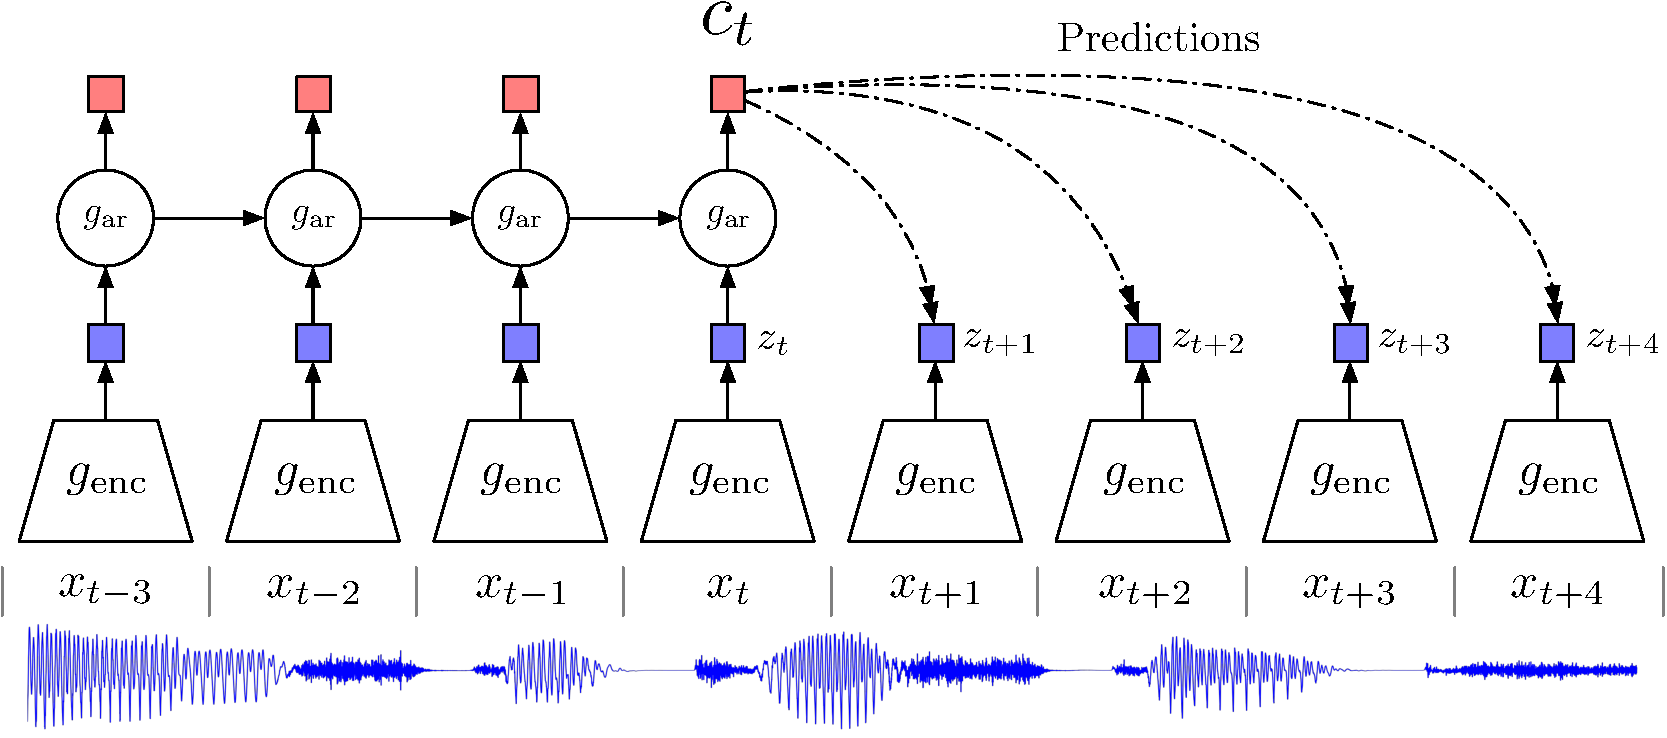
\includegraphics[scale=0.38]{contrastive_repr4.pdf}
    \end{figure}

    \begin{itemize}
      \item \(x_{t_j}\) es la entrada a la red en el instante de tiempo \(t_j\).
      \item \(g_{enc}\) es un codificador que produce una representación \(g_{enc}(x_t) = z_t\)
      \item \(g_{ar}\) es un modelo autorregresivo que produce una representación que tiene en cuenta el contexto \(g_{ar}(z_{\leq t})= c_t\)
    \end{itemize}

      

  
  \end{frame}

  
  \begin{frame}{Pérdida contrastiva y cota inferior contrastiva}
    
    \begin{defi}[Pérdida contrastiva]
      Sea \(X =\{x^*,x_1,\dots,x_{N-1}\}\) un conjunto de \(N\) ejemplos donde $x^*$ ha sido extraido de la distribución conjunta \(P(x,z)\) y le resto han sido extraídos del producto de las distribuciones marginales \(P(x),P(z)\). Se define entonces la función de pérdida contrastiva como  
      \[ 
        \ell(\theta) = - E_X \left[ \log \frac{h_\theta(x^*,z)}{\sum_{x \in X}h_\theta(x,z)}\right]. 
        \]
    \end{defi}

    \pause
    \begin{prop}
      En las mismas condiciones que en la definición anterior, se tiene que
      \[
        I(x^*,z) \geq -  \ell(\theta) + \log N.
      \]
    \end{prop}
  
  \end{frame}
  
  \begin{frame}{Funciones de pérdida usando tripletas}
    \begin{figure}[H]%!htb]
      \minipage{0.32\textwidth}
      \centering
      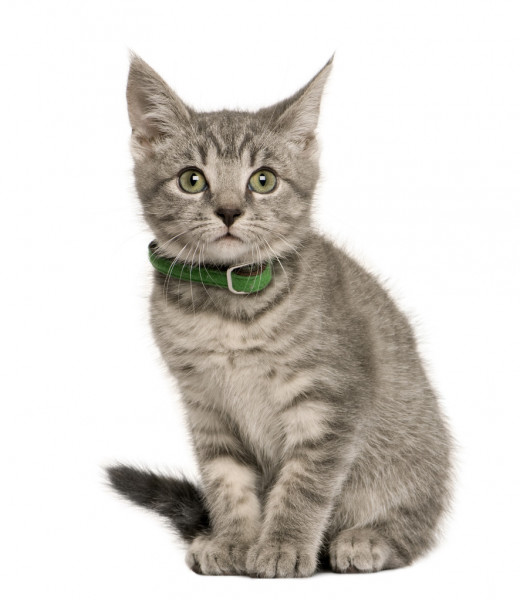
\includegraphics[scale=0.15]{c1}
      \caption*{Original $x$}\label{fig:cat1}
      \endminipage\hfill
      \minipage{0.32\textwidth}%
      \centering
      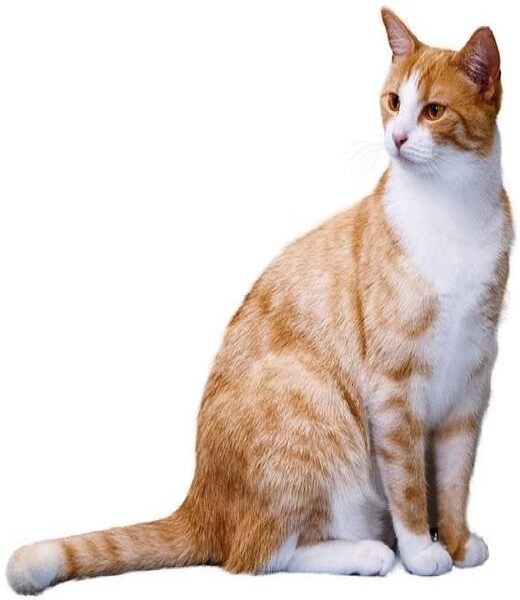
\includegraphics[scale=0.1]{c2}
      \caption*{Ejemplo positivo $\ps$}\label{fig:c2}
      \endminipage
      \minipage{0.32\textwidth}%
      \centering
      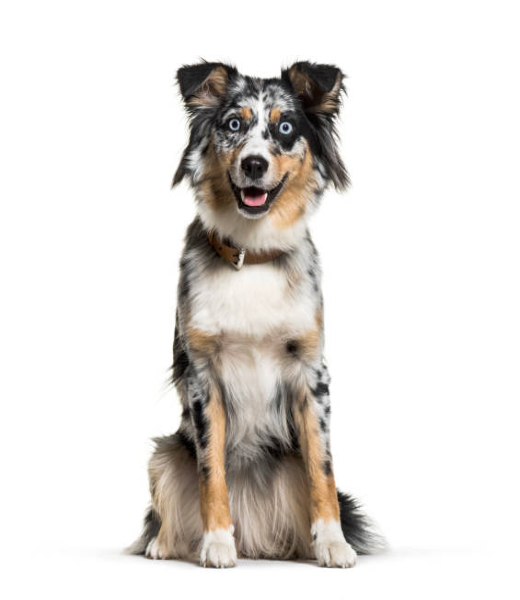
\includegraphics[scale=0.1]{doggo}
      \caption*{Ejemplo negativo $\ns$}\label{fig:doggo}
      \endminipage
    \end{figure}

    Nos interesa tener un margen \(\alpha \in \R\)
    \[
    \norm{g(x) - g(\ps)}_2 + \alpha < \norm{g(x) - g(\ns)}_2,
    \]
    lo que nos lleva a la pérdida de una tripleta individual
    \[
      \ell^\alpha (x,\ps,\ns) = \max \left(0, \norm{g(x) - g(\ps)}_2^2 - \norm{g(x) - g(\ns)}_2^2 + \alpha\right).
    \]

  \end{frame}
  
  \begin{frame}{Funciones de pérdida usando tripletas}


    \begin{defi}
      Dado un conjunto de tripletas, cada una con una imagen original, un ejemplo positivo y uno negativo  \(\mathcal T = \{(x_i,\ps_i,\ns_i)\}_{i \in \Lambda} \), una función de pérdida usando tripletas se define como:
      \[
      \mathcal L (x_i,\ps_i,\ns_i) = \sum_{i \in \Lambda} \ell^\alpha(x_i,\ps_i,\ns_i).
      \]



    \end{defi}
    
    
    Podemos generalizar esta función de pérdida a un caso más eficiente y, a continuación, se puede probar que se está generalizando la pérdida contrastiva.
    
  
  \end{frame}

  \section{Nuevos marcos de trabajo}
  
  \begin{frame}{SimCLR}
    \begin{figure}[H]
      \small
          \centering
      \begin{tikzpicture}
          \node at (0,1.8) (h) {$\longleftarrow\,$Representation$\,\longrightarrow$};
          \node[draw, circle] at (0,-1) (x) {$\,~\bm{x}~\,$};
          \node[draw, circle] at (-2.5,0) (x1) {$\tilde{\bm{x}}_i$};
          \node[draw, circle] at (2.5,0) (x2) {$\tilde{\bm{x}}_j$};
          \node at (-2.5,1.8) (h) {$\bm h_i$};
          \node at (2.5,1.8) (c) {$\bm h_j$};
          \node at (-2.5,3) (hh) {$\bm z_i$};
          \node at (2.5,3) (cc) {$\bm z_j$};
          \path[->] 
              (x)  edge [>=latex] node[below,rotate=-25] {$t\sim\mathcal{T}$} (x1)
              (x)  edge [>=latex] node[below,rotate=25] {$t'\sim \mathcal{T}$} (x2)
              (x1)  edge [>=latex] node[left,rotate=0] {$f(\cdot)$} (h)
              (x2)  edge [>=latex] node[right,rotate=0] {$f(\cdot)$} (c)
              (h)  edge [>=latex] node[left,rotate=0] {$g(\cdot)$} (hh)
              (c)  edge [>=latex] node[right,rotate=0] {$g(\cdot)$} (cc);
          \path[<->]
              (hh)  edge [>=latex] node[above,rotate=0] {Maximize agreement} (cc);
      \end{tikzpicture}
      \end{figure}

      \[
        \ell_{i,j} = -\log \frac{exp(sim(z_i,z_j)/\tau)}{\sum_{k=1}^{2N} I_{k \neq i} exp(sim(z_i,z_k)/\tau)},    
      \]
  \end{frame}

  
  \begin{frame}{Bootstrap your own latent}
    \begin{figure}[H]
      \centering 
      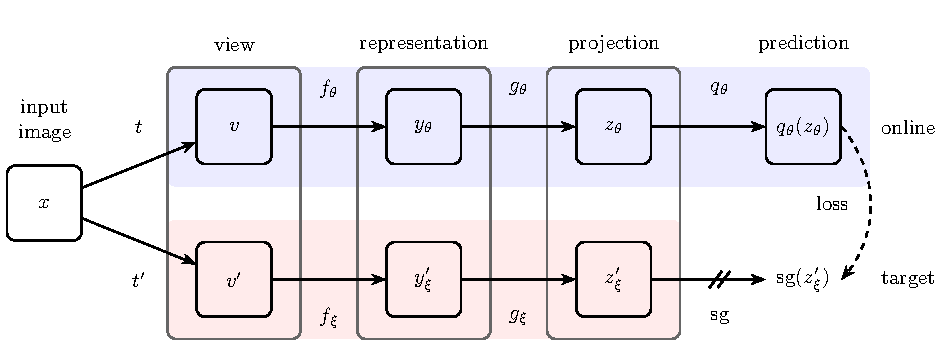
\includegraphics[scale=0.8]{Archi-BYOL.pdf}
    \end{figure}

    \[
    \mathcal L_{\theta,\upxi} = \norm{\overline{q_\theta}(z_\theta) - \overline{z_\upxi'}}_2^2 
    \]
    \[
    \upxi \gets \tau \upxi + (1-\tau) \theta  
    \]
  \end{frame}

  \section{Experimentos}
  
  \begin{frame}{Problemas y objetivos}
    \textbf{Problemas:}
    \pause
    \begin{itemize}
      \item El conjunto de datos usado en los artículos originales es demasiado grande
      \pause
      \item La capacidad de la que disponemos es claramente inferior (1GPU vs 128 TPU)
    \end{itemize}

    \pause

    \textbf{Objetivos:}
    \begin{itemize}
      \item Adaptar los experimentos a un conjunto de datos más pequeño
      \pause
      \item Experimentar con los hiperparámetros de los modelos para comprobar si las hipótesis originales se siguen cumpliendo
    
    \end{itemize}

    \pause
    \textbf{Tecnologías (Python):}
    \begin{itemize}
      \item Tensorflow
      \item Jax
      \item Tensorboard
    \end{itemize}
  \end{frame}

  
  \begin{frame}{Primer experimento SimCLR}
  Primer acercamiento, búsqueda en malla para explorar el comportamiento de los hiperparámetros:
  \pause

  \begin{itemize}
   \item Tamaño de batch 
   \item Temperatura $\tau$
   \item Intensidad de la fluctuación de color
  \end{itemize}
  \pause

  Este primer experimento se hace utilizando \textbf{ResNet18} como codificador.
  \pause



  \begin{table}[H]
\centering
\resizebox{\columnwidth}{!}{
\begin{tabular}{lrrrrrr}
Procedencia & batch\_size   & temperature   & color\_jitter & regularization\_loss & top\_1\_accuracy & top\_5\_accuracy          \\ \hline
 Propio &512  &  0.25 &  0.25 &  0.0093      &  0.833         &  0.994          \\
 Propio &1024 &    0.25       &  0.75 &  0.0093      & 0.841          &  0.995           \\ \hdashline
 Original & 512 & 0.5 & - & - & $\sim 0.846$ & -  \\
 Original & 1024 & 0.5 & - & - &  $\sim 0.851$ & - \\
\end{tabular}
}
\end{table}
  

  \end{frame}

  
  \begin{frame}{Influencia del tamaño de batch }

    \begin{figure}[htp] 
      \centering
      \subfloat[Evolución de la precisión según el tamaño del batch.]{%
          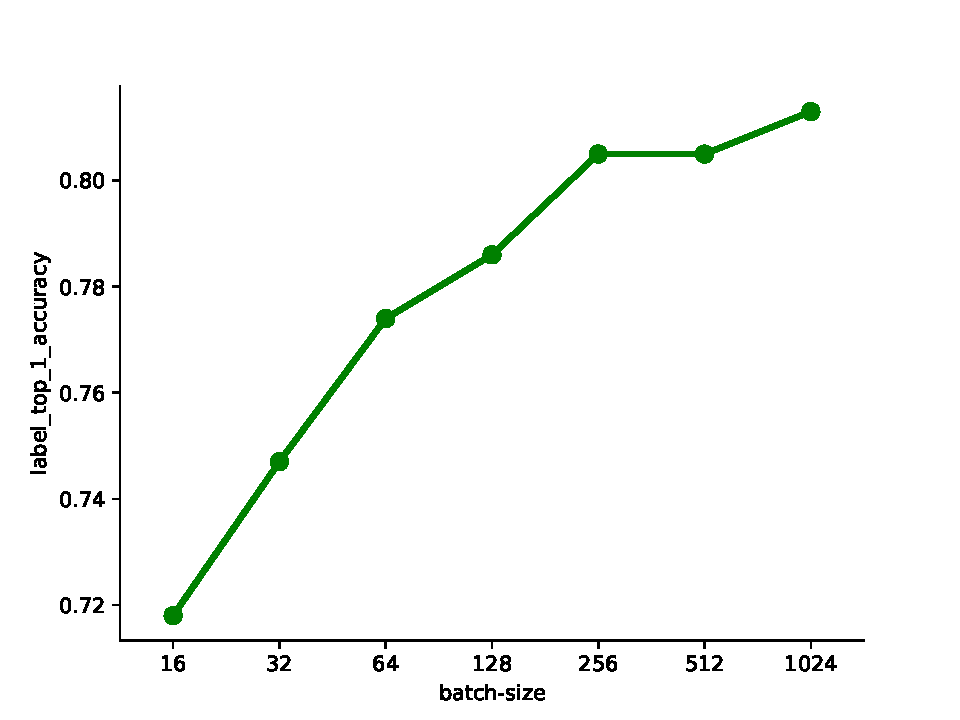
\includegraphics[width=0.45\textwidth]{simclr-batch-comparison}%
          }%
      \hfill%
      \subfloat[Curvas de evolución de la precisión en función del tamaño del batch.]{%
          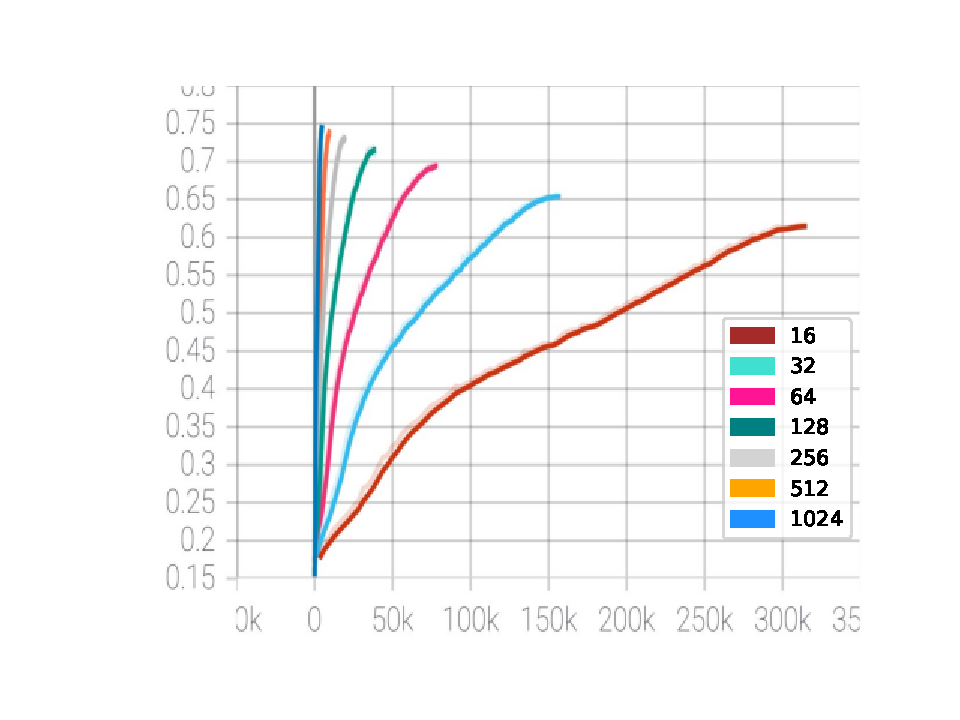
\includegraphics[width=0.45\textwidth]{train_supervised_acc}%
        
  
          }%
  \end{figure}

  En la evaluación de la pérdida, se compara con el resto del batch.
  \end{frame}

  
  \begin{frame}{Influencias de la intensidad de fluctuación del color y de la temperatura}

    \begin{figure}[htp] 
      \centering
      \subfloat[Influencia de la intensidad de fluctuación.]{%
      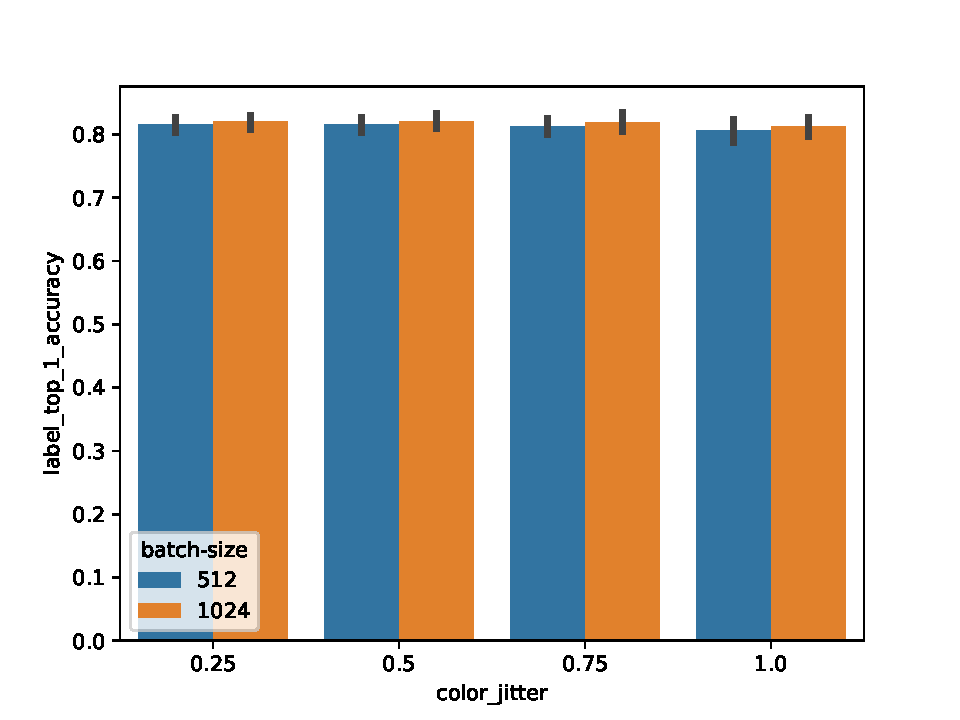
\includegraphics[width=0.48\textwidth]{color-jitter-impact-simclr}%
          %
          }%
      \hfill%
      \subfloat[Influencia de la temperatura.]{%
          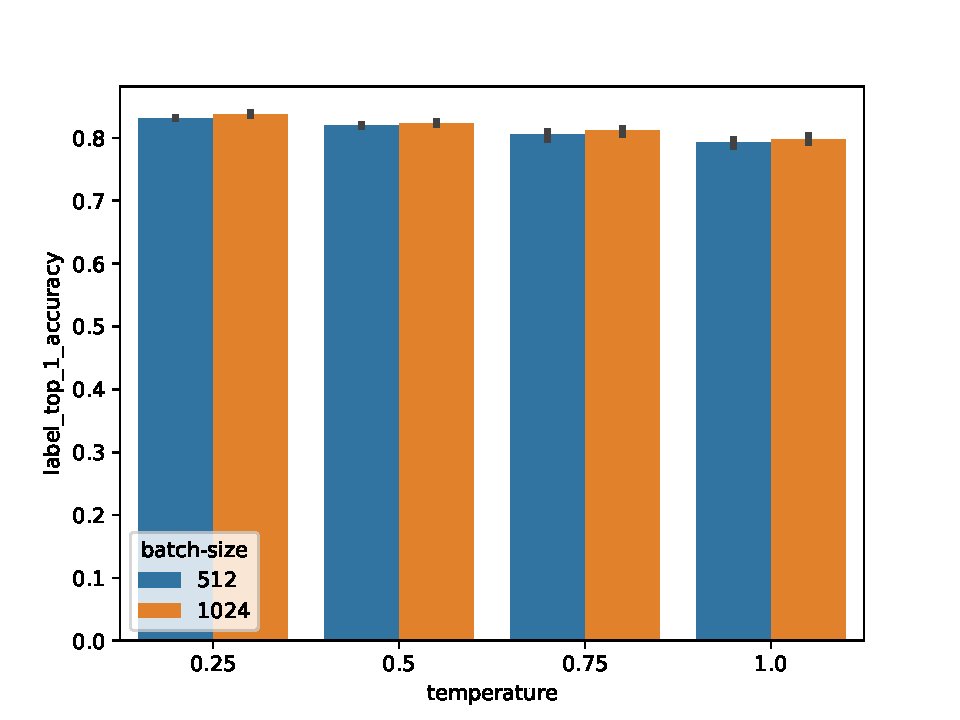
\includegraphics[width=0.48\textwidth]{temperature-impact-simclr}
          
  
          }%
  \end{figure}

  
  \end{frame}

  
  \begin{frame}{Segundo experimento SimCLR}
  Aumentamos la profundidad del codificador, usamos \textbf{ResNet50}.

  \begin{figure}[htp] 
    \centering
    \subfloat[Pérdida contrastiva en train]{%
        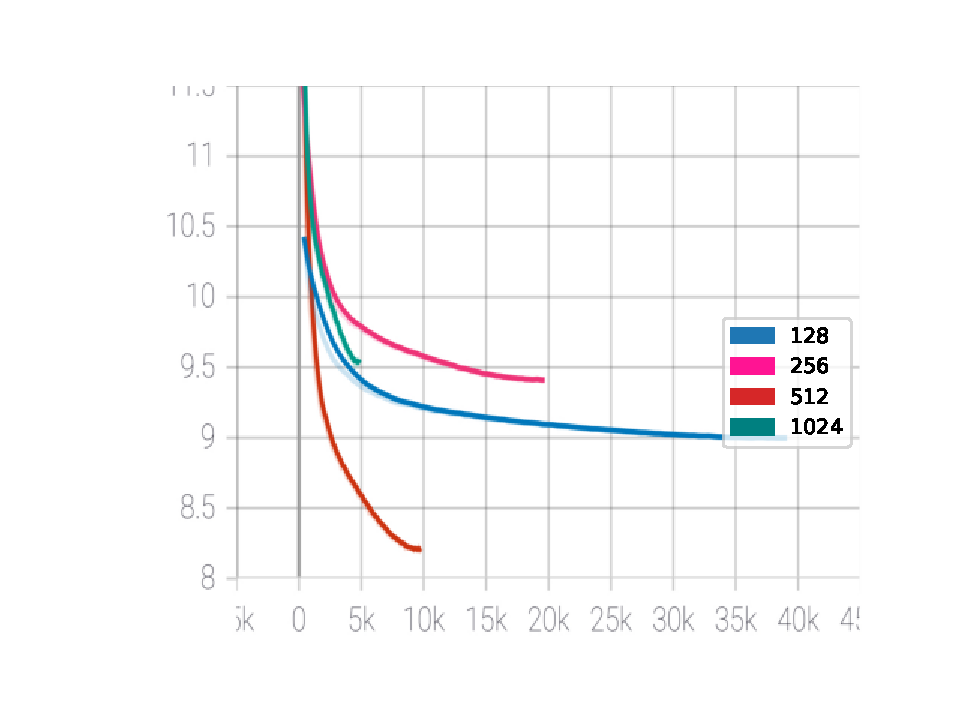
\includegraphics[width=0.3\textwidth]{simclr-exp2/train_contrast_loss}%
        %
        }%
    %
    \subfloat[Pérdida supervisada]{%
        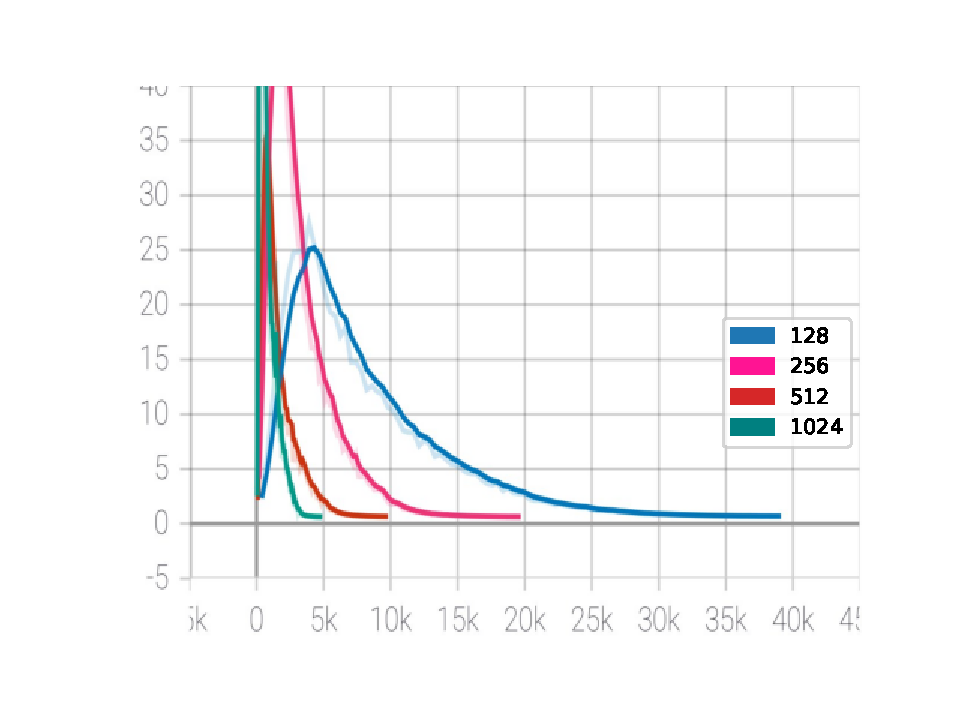
\includegraphics[width=0.3\textwidth]{simclr-exp2/train_supervised_loss}%
        

        }%
        \begin{table}[H]
          \centering
          \resizebox{\columnwidth}{!}{
          \begin{tabular}{rlllllll}
          resnet\_depth & batch\_size   & temperature   & color\_jitter & regularization\_loss & top\_1\_accuracy & top\_5\_accuracy & steps         \\ \hline
          18 & 1024 &    0.25       &  0.75 &  0.0093      &  0.841          &  0.995          &  4900 \\
          \textbf{50} & 128 & 0.5 & 0.65 & 0.0225 & 0.844 & 0.994 & 39100 \\
           & \textbf{256} & \textbf{0.5} & \textbf{0.75} & \textbf{0.023} & \textbf{0.848} & \textbf{0.994} & \textbf{19695} 
          \end{tabular}
          }
          
          \label{table:best:second:simclr}
          \end{table}
      
\end{figure}

  
  \end{frame}

  
  
  \begin{frame}{Tercer experimento y resultados finales}
  Añadimos \textbf{alisado gaussiano} al preprocesamiento.
  \begin{table}[H]
    \resizebox{\columnwidth}{!}{
    \begin{tabular}{rrrrrrrrr}{}
    Experimento &resnet\_depth & batch\_size  & temperature   & color\_jitter & regularization\_loss & label\_top\_1\_accuracy & label\_top\_5\_accuracy & global\_step   \\ \hline 
1& 18 & 1024 &    0.25       &  0.75 &  0.0093      &  0.841          &  0.995          &  4900 \\
2& 50 & {256} & {0.5} & {0.75} & {0.023} & {0.848} & {994} & {19695}  \\
\textbf{3}&    18              & 1024         & 0.25          & 0.65          & 0.0093               & 0.846                   & 0.994   &  4900                     \\
& \textbf{50}   & \textbf{256} & \textbf{0.25} & \textbf{0.65} & \textbf{0.0228}      & \textbf{0.862}          & \textbf{0.997} & \textbf{19695}\\
 \hdashline
 Original & 50&  512 & 0.5 & - & - & $\sim 0.846$ & - & 9800 \\
  & 50&1024 & 0.5 & - & - &  $\sim 0.851$ & - & 4900\\                                                    
    \end{tabular}
    }
    \end{table}
  
    \pause

    \begin{shaded}
      Encontramos un \textbf{bug} en el código de Google a la hora de realizar la transferencia de aprendizaje a otros dataset.
    \end{shaded}
  \end{frame}

  
  
  \begin{frame}{Experimento con BYOL}

  Se pretende comprobar (usando \textbf{ResNet50}) si el tamaño de batch sigue siendo relevante y si se obtienen mejores resultados que los obtenidos en SimCLR.

\begin{columns}
  \begin{column}{0.4\textwidth}
    \[
      \mathcal L_{\theta,\upxi} = \norm{\overline{q_\theta}(z_\theta) - \overline{z_\upxi'}}_2^2 
      \]
  \end{column}
  \pause
  \begin{column}{0.6\textwidth}  %%<--- here
    \begin{figure}[H]
      \centering 
      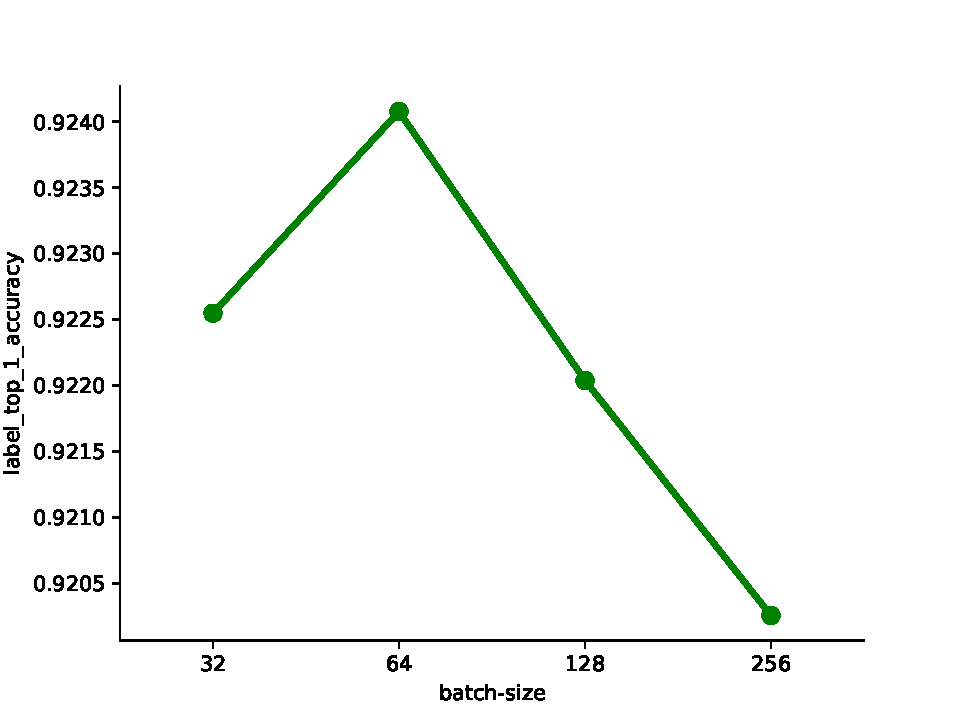
\includegraphics[scale=0.3]{byol-batch-comparison}
    \end{figure}
  \end{column}
\end{columns}


\begin{table}[H]
  \resizebox{\columnwidth}{!}{
  \begin{tabular}{rrrrr}
  batch\_size  & loss & top\_1\_accuracy & top\_5\_accuracy & steps    \\ \hline
  
  \textbf{64} & \textbf{0.381}       & \textbf{0.9240764}          & \textbf{1}              & \textbf{148000} \\       
  \end{tabular}
  }
  \end{table}

  
  
  
  \end{frame}
  

  


  
  \begin{frame}{Conclusiones}

    \begin{itemize}
      \item El uso de la teoría de la información proporciona un buen punto de partida para el aprendizaje de representaciones.
      \item El aprendizaje contrastivo ha probado ser la mejor forma de obtener representaciones que son útiles en tareas posteriores.
      \item Ambos marcos de trabajo probados obtienen buenos resultados en la adaptación a conjuntos de datos más pequeños.
    \end{itemize}
  \end{frame}
  
  \appendix

  \begin{frame}[noframenumbering,standout]
    Gracias por su atención
  \end{frame}

  
  \begin{frame}[noframenumbering]{Nota final}
    El contenido que se expondrá en esta presentación está explicado detalladamente en un documento en
    \begin{center}
    \url{https://github.com/fjsaezm/Mutual-Information-in-Unsupervised-Machine-Learning}.
    \end{center}

    El código que se ha elaborado para ayudarnos en este trabajo también se encuentra en este repositorio.
    
  \end{frame}


\end{document}
